\chapter{Data Visualization}
For preparing data for data mining task it is essential to have an overall picture of your data, so we have to
gain insight in your data, with respect to your project goals and should be general to understand properties.\newline
You should discover semantics of data and also to discover statistical charecteristics of your data in
order to have a more understanding of data.

Data can be represent usually by $3$ modes:
\begin{itemize}
    \item Record: we have a matrix representation that will represent data and it is divided in:
            \begin{itemize}
                \item Data Matrix: If data objects have the same fixed set of numeric attributes,
                      then the data objects can be thought of as points in a multidimensional space,
                      where each dimension represents a distinct attribute.\newline
                      Such data set can be represented by an $m$ by $n$ matrix, where there are $m$ rows,
                      one for each object, and $n$ columns, one for each attribute.

                \item Document Matrix: each document becomes a ‘term’ vector, where each term 
                      is a component (attribute) of the vector and the value of each component is 
                      the number of times the corresponding term occurs in the document.
                \item Transiction Data: A special type of record data, where each record (transaction)
                      involves a set of items, so for example consider a grocery store.\newline
                      The set of products purchased by a customer during one shopping trip constitute a transaction,
                      while the individual products that were purchased are the items,
                      as it possible to note in figure \ref{img:transiction}.
            \end{itemize}
    \item Graph
    \item Order
\end{itemize}

\begin{figure}
    \caption{Example of Transiction Data}
    \label{img:transiction}
    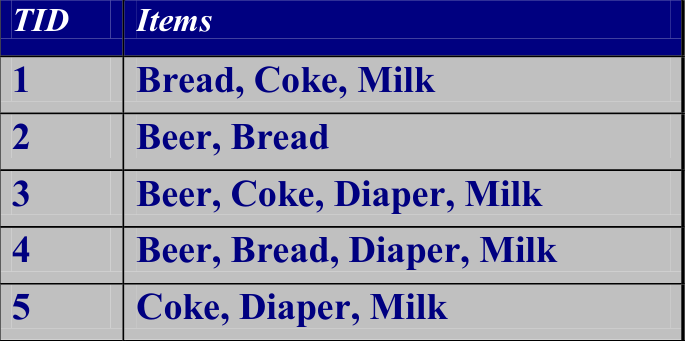
\includegraphics[width=\textwidth]{Images/transiction}
\end{figure}
Data is a collection of data objects and their attributes, where the last one is a property or 
characteristic of an object like eye color of a person and a data object is a collection of 
attributes that descrive an object.

There are different types of attributes:
\begin{description}
    \item [Nominal/Categorical: ] attribute values in a finite domain, categories, “name of things” like
                                  eye color, zip codes.
    \item [Binary: ] nominal attribute with only $2$ states ($0$ and $1$) where we have \emph{symmetric binary},
                     in which both outcomes are equally important, or also \emph{asymmetric binary} where 
                     outcomes are not equally important, like medical test positive vs negative, and the convention
                     is to assign $1$ to most important outcome.
    \item [Ordinal: ] finite domain with a meangniful ordering on the domain, like rankings, grades and height.
    \item [Numeric: ] quantity (integer or real-valued) measured on a scale of equal-sized units and which
                      values have order, example of this data are temperatures in Celsius and calendar dates.
    \item [Ratio-scaled: ] we can speak of values as being an order of magnitude larger than the unit of measurement
                           and example are length, elapsed time and so on.
\end{description}
There is also a distinction about which data an attribute can have:
\begin{description}
    \item [Discrete Attribute: ] has only a finite or countably infinite set of values and often are represented
                                 as integer variables, where we can note that binary attributes are a special
                                 case of discrete attributes.
    \item [Continuous Attribute: ] has real numbers as attribute values and practically real values can only
                                   be measured and represented using a finite number of digits.\newline
                                   Examples are temperature, weight, or height and also continuous attributes
                                   are typically represented as floating-point variables.
\end{description}
The type of an attribute depends on which of the following properties/operations it possesses:
\begin{description}
    \item [Distinctness: ] $= \neq$
    \item [Order: ] $< >$
    \item [Differences: ] are $+ -$
    \item [Ratios: ] are $* /$
\end{description}
We have that Nominal attribute has only distinctness, ordinal attribute add the order property, interval
attribute has also differences and in the end ratio attribute has all $4$ properties.

Poor data quality negatively affects many data processing efforts infact we have that the most important point
is that poor data quality is an unfolding disaster and also poor data quality costs to a typical company
at least $10\%$ of revenue, but $20\%$ is probably a better estimate.

Some \emph{Data quality} issues are the following:
\begin{description}
    \item [Syntactic accuracy: ] entry is not in the domain, like write "fmale" in gender, and that can be 
                                  checked and solve quite easy.
    \item [Semantic accuracy: ] entry is in the domain but not correct, like "Bergamo is in France", and 
                                that type of error needs more information to be checked ("business rules").
    \item [Completeness: ] is violated if an entry is not correct although it belongs to the domain of the attribute,
                           and that happens when complete records are missing so the data is biased.

    \item [Unbalanced data: ] the data set might be biased extremely to one type of records.
    \item [Timeliness: ] is the available data up to date?
\end{description}
Data set may include data objects that are duplicates, or almost duplicates of one another and that is 
a major issue when we are merging data from heterogeneous sources, an example can be a same person with
multiple email addresses.
\emph{Data cleaning} is the process of dealing with duplicate data issues and consists to discover 
missing data and outlier with the purpose to remove all or at least a largest part.

In figure \ref{img:rescale} we can see that in $2001$ there was the change from Lira to Euro and 
that explain a dramatic reduction on a problem so we have to rescale values that makes consistent data.

\begin{figure}
    \caption{Change of scale in Revenue in Italy}
    \label{img:rescale}
    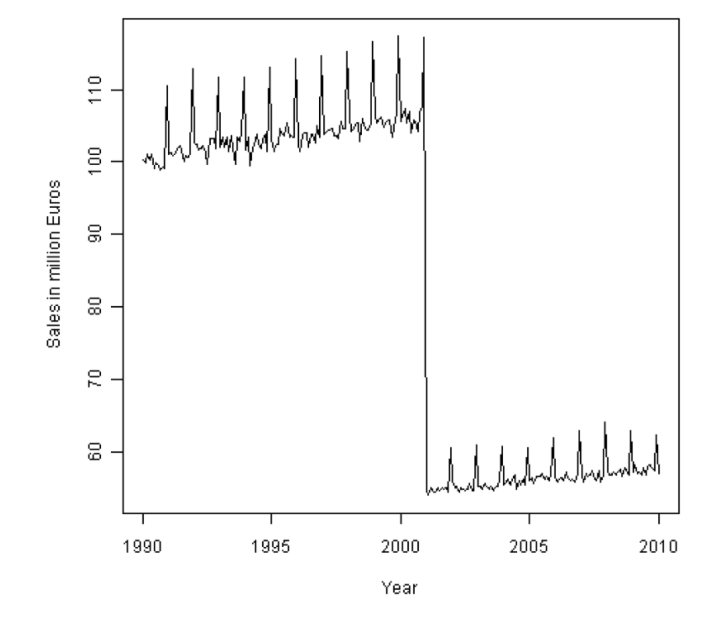
\includegraphics[width=\textwidth]{Images/rescale}
\end{figure}

The distribution of data observation is important to recognize if we have symmetric data, skewed data, bimodal
pattern (which usually shows subpopulation on attribute) and when visualisations reveal patterns or exceptions,
then there is “something” in the data set; when visualisations do not indicate anything specific,
there might still be patterns or structures in the data that cannot be revealed by the corresponding
(simple) visualisation techniques.


We will define now what we intend when we talk about outlier:
\begin{defi}
    Outliers are data objects with characteristics that are considerably different than most of the other
    data objects in the data set.
\end{defi}
There are two different cases: one when Outliers are noise that interferes with data analysis and another
when Outliers are the goal of our analysis, like in credit card fraud and intrusion detection.\newline
Outliers cause data quality problems and should be exceptional or an unusual data objects, so 
outliers coming from erroneous data should be excluded from the analysis and even if the outliers are correct
(exceptional data), it is sometime useful to exclude them from the analysis.\newline
For example, a single extremely large outlier can lead to completely misleading values for the mean value.

To detect an outlier we can do the following actions:
\begin{description}
    \item [Single Attribute: ] when we have an outlier in categorial attributes we can find it when we have 
                               a value that occurs with an extremely lower frequency than other; in case we 
                               want to discover an outlier in numerical attributes we use box plots.
    \item [Multidimensional Attribute: ] we can use Scatter plots for visually detect outliers for two attributes or
                                         also we can use PCA or MDS plots to discover outliers.
\end{description}
For some instances values of single attributes might be missing, due to a missing a collection of an information,
broken sensors and also attributes may not be applicable to all cases, and also missing value might not
necessarily be indicated as missing, we can use instead zero or default values.

\section{Data Preparation}
Data preparation uses informations from data understanding to select attributes, reduce the data dimension,
select records, treat missing values, treat outliers, integrate, unify and transform data 
and in the end we can improve data quality.

In Data Preparation can be execute the following operations:
\begin{description}
    \item [Aggregation: ] combining two or more attributes (or objects) into a single attribute (or object)
                          with the purpose of reduce the number of attributes/objects, have more stable
                          data and also to change the scale, like aggregate cities into regions.\newline
                          In figure \ref{img:stableData} it is possible that aggregation from number of precipitation
                          from a month in Australia in number of precipitation in a year make more stable data.
                          \begin{figure}
				  \caption{Example Aggregation on Australia's precipitation}
                              \label{img:stableData}
			      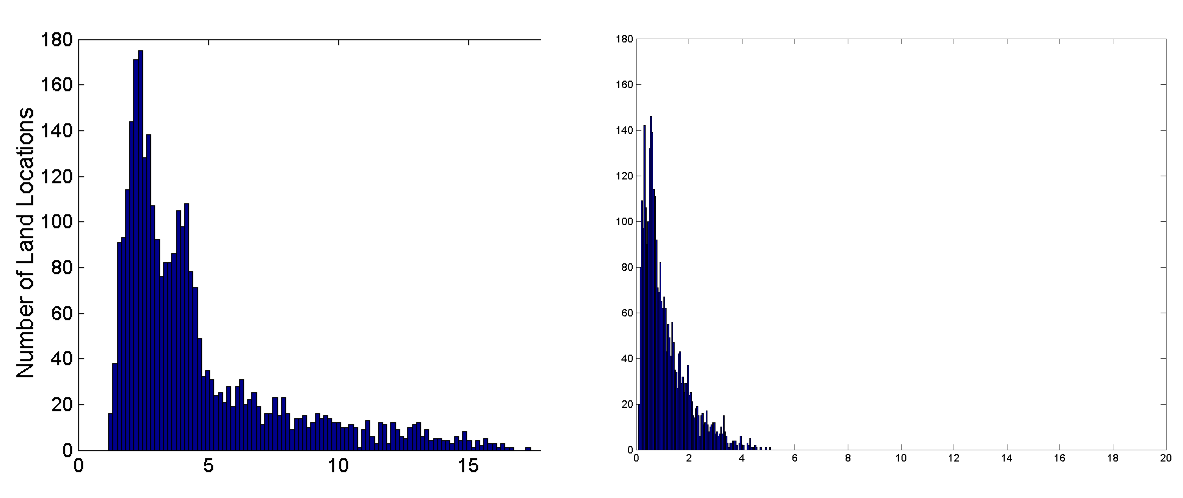
\includegraphics[width=\textwidth]{Images/stableData}
                          \end{figure}
    \item [Data Reduction: ] we reduce the amount of data that can be done in two ways:
                             \begin{itemize}
                                \item Reduce the number of records, using Data Sampling and Clustering.
                                \item Reduce the number of columns (attributes), where we select a subset
                                      of attributes and we generate a new (a smaller) set of attributes
                             \end{itemize}
                             \emph{Sampling} is the main technique employed for data reduction and it
                             is often used for both the preliminary investigation of the data 
                             and the final data analysis.\newline
                             Sampling is typically used in data mining because processing the entire set of data
                             of interest is too expensive or time consuming.

                             The key principle for effective sampling is to using a sample that will work
                             almost as well as using the entire dataset, if the sample is \emph{representative},
                             that happens if the same has approximately the same properties as 
                             the original set of data.
                            
                             The types of Samplings are the following:
                             \begin{description}
                                 \item [Simple Random Sampling: ] there is an equal probability of selecting
                                        any particular item and we can have sampling without and with replacement.
                                 \item [Stratified Sampling: ] split the data into several partitions and 
                                        then draw random samples from each partition and we create an
                                        approximation of the percentage of each class; it is suitable 
                                        for distribution with peaks, in which each peak is a layer.
                             \end{description}
    \item [Dimension Reduction: ] selection of a subset of attributes that is as small as possible
                                  and sufficient for the data analysis.\newline
                                  Consist in removing (more or less) irrelevant features, that contain no 
                                  information useful for data mining (students ID is irrelevant in predicting 
                                  student GPA), and also removing redundant features, that duplicate much or 
                                  all of the information contained in one or more other attributes.\newline
                                  When dimensionality increases, data becomes increasingly sparse in the
                                  space that it occupies(curse of dimensionality) and also definitions of
                                  density and distance between points, which are critical for clustering
                                  and outlier detection, become less meaningful.

                                  The reduction of dimension has the purpose to avoid curse of dimensionality,
                                  reduce amount of time and memory required by datamining algorithms, 
                                  allow data to be more easily visualized and 
                                  may help to eliminate irrelevant features or reduce noise.

                                  It uses PCA(Principal Components Analysis), Singular Value Decomposition
                                  or other supervised and non-linear techniques.
                                
                                  For removing irrelevant features, a performance measure is needed that
                                  indicates how well a feature or subset of features performs and for removing
                                  redundant features, either a performance measure for subsets of features or a
                                  correlation measure is needed.

                                  To reduce the dimension we usually use these $3$ methods:
                                  \begin{description}
                                      \item [Filter Method: ] selection after analyzing the significance and 
                                                              correlation with other attributes (preprocessing)
                                      \item [Wrapper Method: ] selecting the top-ranked features using 
                                                               as reference a DM task and there is an incremental
                                                               selection of the “best” attributes, with respect
                                                               of information gain.
                                      \item [Embedded Method: ] selection as part of the data mining algorithm,
                                                                so during the operation of the DM algorithm,
                                                                the algorithm itself decides which attributes to use
                                                                and which to ignore, like Decision tree.
                                  \end{description}
    \item [Feature Creation: ] create new attributes that can capture the important information in a dataset
                               much more efficiently than the original attributes and 
                               there are two general methodologies:
                               \begin{itemize}
                                   \item Feature construction: in figure \ref{img:featureCreation} can be seen
                                         an example on how to create a new feature.
                                   \item Feature projection: it transforms the data in the high-dimensional space
                                         to a space of fewer dimensions and this transformation may be linear,
                                         or nonlinear.\newline
					 It uses PCA (Principal Component Analysis), SVD (Singular Value Decomposition),
					 Autoencoder and LDA (Linear Discriminant Analysis).
                               \end{itemize}

                               \begin{figure}
                                    \caption{Example of Feature Creation}
                                    \label{img:featureCreation}
                                    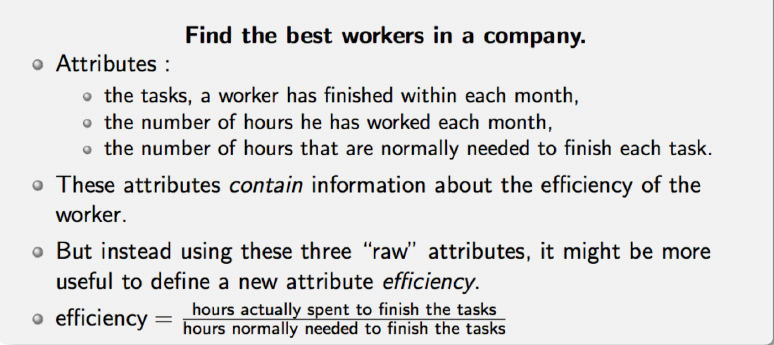
\includegraphics[width=\textwidth]{Images/featureCreation}
                               \end{figure}
\end{description}
\emph{Data Cleaning} will deal on how to handle anomalous values, how to handle outliers and also on data transformations, so we will
start to discuss on how we can manage missing values: a first approach can be to eliminate records that contain missing values or also it 
is possibile to substitute values, estimate using a probability distribution of existing values or also build a model (regression/classification) 
for computing missing values, or even using mean, median and mode.

\emph{Discretization} is the process of converting a continuous attribute into an ordinal attribute, where potentially infinite number of values
are mapped into a small number of categories and this technique is commonly used in classification, because many classification algorithms 
work best if both the independent and dependent variables have only a few values.\newline
The advantages of Discretization is that original values can be continuous and sparse instead discretized data can be simple to be interpreted 
and also data distribution after discretization can have a normal shape.

There are two different approach to discretize data:
\begin{description}
   \item [Unsupervised Discretization: ] we don't have label for the instances and the number of classes is unknown and there are 3 technique to bin data:
	   				 \begin{description}
					     \item [Natural Binning: ] it is a simple approach, which subdivise sorted attributes values in $k$ parts
						                       with the same  size using a interval size defined as 
						                       \[ \delta = \frac{x_{max} - x_{min}}{k} \]
								       so an element $x_j$ belong to a class $i$ if 
								       \[ x_j \in (x_min + i \delta, x_min + (i + 1) \delta) \]
								       The problem of this approach is that can generate distribution very unbalanced.
					     \item [Equal Frequency Binning: ]  we sort, count the elements, and we define $k$ intervals of $f$ as 
						     				\[ f = \frac{N}{k} \]
										where $N$ are the number of elements on the sample.\newline
										An element $x_j$ belongs to a class $j$ if we have 
										\[ j \times f \leq i \leq (j + 1) \times f \]
										It is not always suitable for highlighting interesting correlations.
					     \item [Statisical Binning: ] it uses statistical information (Mean, variance, quartile) to create $k$ interval
					\end{description}
					The optimal number of classes is function of $N$ elements defined by \cite{sturges} in $1929$
					\[ C = 1 + \frac{10}{3} \log _{10} N \]
					and the optimal width of the classes depends on the variance and the number of data as told in $1979$ in \cite{scott}
					\[ h = \frac{3.5 * s}{\sqrt{N}} \]

    \item [Supervised Discretization: ] the discretization has a quantifiable goal and the number of classes is known and there are two techniques used:
	    				\begin{itemize}
					    \item discretization based on percentiles
					    \item discretization based on \emph{Entropy}: Minimizes the entropy of a label, that maximizes the purity of the
					          intervals, so in this starts by bisecting the initial values so that the resulting two intervals
						  give minimum entropy, the splitting process is then with another interval, typically
						  choosing the interval with the worst (highest) entropy and in the end we will stop when a user-specified 
						  number of intervals is reached, or a stopping criterion is satisfied.
					\end{itemize}
\end{description}
\emph{Binarization} maps a continuous or categorical attribute into one or more binary variables and it is typically used for association analysis.\newline
We often convert a continuous attribute to a categorical attribute and then convert a categorical attribute to a set of binary attributes.

\section{Data Transformation}
In this section we will briefly talk about data transformation that can reduce in particular two issues: data with errors and imcomplete and 
data not adequately distributed (with many peaks and strong asymmetry in the data).

An \emph{attribute transform} is a function that maps the entire set of values of a given attribute to a new set of replacement values such that
each old value can be identified with one of the new values.\newline
It can be done by a simple function ($e^x, \log x$ for example) or by normalization and in statistics standardization refers to substracting off
the means and dividing by the standard deviation.\newline
We define a transformation $T$ on the attribute $X$ as $Y = T(X)$ such that $Y$ preserve the relevant information of $X$, $Y$ is more useful of $X$ and 
in the end $Y$ eliminates at least one of the problems of $X$.

The goals of data transformation are the following:
\begin{itemize}
    \item stabilize the variances
    \item normalize the distributions
    \item make linear relationships among variables
    \item simplify the elaboration of data containing features you do not like
    \item represent data in a scale considered more suitable
\end{itemize}
To normalize data there are $3$ techniques that are the following:
\begin{description}
    \item [Min-Max normalization: ] we transform data using a new max e min of our data as following
	    			    \[ v' = \frac{v - min_A}{max_A - min_A} (new\_max_A - new\_min_A) + new\_min_A \]
    \item [Z-score normalization: ] we transform to a variable distributed as a $Z$ with the following transformation
	                            \[ v' = \frac{(v - mean_A)}{stdev_A} \]
    \item [Decimal scaling: ] we scale all values $V$ by a decimal scaling defined as
	                      \[ v' = \frac{v}{10^j} \]
			      where $j$ is the smallest number such that $max |v'| \leq 1$.
\end{description}


\section{PCA: Principal Component Analysis}
The goal of PCA is to find a new set of dimensions (attributes or features) that better captures the variability of the data and in PCA
the first dimension is chosen to capture as much of the variability as possible; the second dimension is orthogonal to the first
and, subject to that constraint, captures as much of the remaining variability as possible, and so on.\newline
It is a linear transformation that chooses a new coordinate system for the data set and the steps done in PCA approach are the following:
\begin{enumerate}
    \item Standardize the dataset 
    \item Calculate the covariance matrix for the features in the dataset.
    \item Calculate the eigenvalues and eigenvectors for the covariance matrix.
    \item Sort eigenvalues and their corresponding eigenvectors and pick $k$ eigenvalues and form a matrix of eigenvectors. 
    \item Transform the original matrix.
\end{enumerate}
PCA calculates the covariance matrix of all pairs of attributes given matrix D of data, where remove the mean of each column from the column vectors
to get the centered matrix $C$ (standardization) and then compute the matrix $V = \transpose{C} C$, the covariance matrix of the row vectors of $C$.

Exact value in Covariance matrixis not as important as it’s sign, so a positive value of covariance indicates both dimensions increase or decrease together,
a negative value indicates while one increases the other decreases, or vice-versa and in the end if covariance is zero 
the two dimensions are independent of each other.

We identify the principal components of data by computing the eigenvectors and eigenvalues from the covariance matrix, these components are 
new variables that are constructed as linear combinations of the initial variables, uncorrelated and most of the information 
within the initial variables is squeezed or compressed into the first components, infact PCA tries to put maximum possible information in the first
component, then maximum remaining information in the second and so on.

The eigenvectors of the Covariance matrix are actually the directions of the axes where there is the most variance(most information) and 
Eigenvalues are simply the coefficients attached to eigenvectors, which give the amount of variance carried in each PC.\newline
By ranking your eigenvectors in order of their eigenvalues, highest to lowest, you get the principal components in order of significance.
